\section{Critère local de collage}
Dans cette partie on montre l'existence de certains clusters avec une bonne probabilité pour relier des parties de~$\Sk$ en vue d'une renormalisation (partie~\ref{sec:renormalisation}). Pour cela, on introduit une suite~$\suite{u}$ telle que~$u_n \leqslant n/3$ et %que (?)
	\begin{equation}\label{eq:toucherBordCarre}
		\Pp{\relie*[B_n]{B_{u_n}}{\partial B_n}} \underset{n \to \infty}{\to} 1. 
	\end{equation}
	Pour s'épargner une écriture trop lourde, on note~$S_n = B_{u_n}$ \marginnote{$S_n$} et on définit, pour~$\alpha, \beta$ des réels de~$[0, n]$, l'événement~$\mathcal{E}_n(\alpha, \beta)$ par
	\[
		\mathcal{E}_n( \alpha, \beta ) = \{\relie[B_n]{S_n}{\{n\} \times \llbracket \alpha ; \beta \rrbracket} \}. \marginnote{$\mathcal{E}_n$}
	\]
	
	\begin{lem}\label{lem:collagesElem} \marginnote{$\alpha_n, y_n$}
		Il existe deux suites~$\suite{\alpha}$ et~$\suite{y}$ dans~$[0; n]$ telles que
		\begin{align*}
			  &\Pp{\mathcal{E}_n(\alpha_n, n)} \xrightarrow[n\to\infty]{} 1 \\ 
			  &\Pp{\mathcal{E}_n\left(y_n - \frac{\alpha_n}{4}, y_n + \frac{\alpha_n}{4}\right)} \xrightarrow[n \to \infty]{} 1.
		\end{align*}
		Ces deux événements sont illustrés dans la figure~\ref{fig:figuLemCollagesElem}
	\end{lem}
	
	\begin{figure}[h]
		\begin{center}
			% L'événement \mathcal{E}_n(\alpha_n, n)
			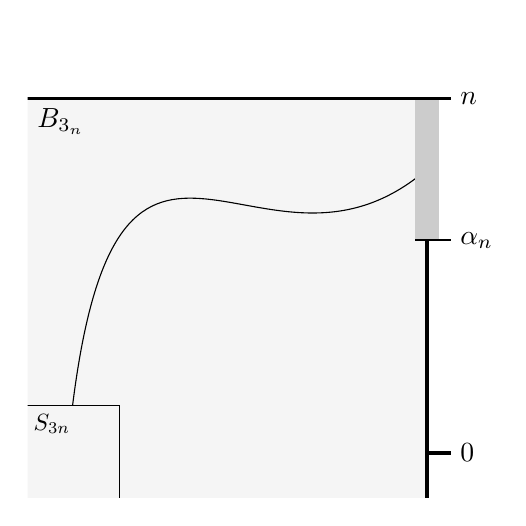
\begin{tikzpicture}[scale = 0.3]
				% Clip
				\clip 					(-1.9,-1.9)	rectangle	(18,18)	;
				% Fond
				\fill [color=gray!8]	(-15,-15)	rectangle	(15,15)	;	% B_n
				% Rectangles
				\draw 	[very thick]	(-15,-15)	rectangle 	(15,15) ;	%B_3n
				\draw 					(-2,-2) 	rectangle 	(2,2) 	;	%S_3n
				% Courbe de Bézier
				\draw (0, 2) 	.. controls (2, 18) and  (8, 6) .. (15, 12);
				% Plage
				\fill [color=gray!40]	(14.5, 9) 	rectangle (15.5, 15);	% \alpha_n
				% Points
				\path [below right]	(-1.9, 15)	node				{$B_{3_n}$}	;
				\path [below right]	(-2, 2)		node	[scale=0.85]{$S_{3n}$}	;
				% Courbes de séparation
				\draw [very thick]	(15, 0)		-- (16, 0);
				\draw [very thick] 	(14, 15) 	-- (16, 15);
				\draw [thick]		(14.5, 9) 	-- (16, 9);
				\draw [right]		(16, 0) 	node {$0$};
				\draw [right]		(16, 9)		node {$\alpha_n$};
				\draw [right]		(16, 15) 	node {$n$};
			\end{tikzpicture}
			\quad \quad
			% L'événement \mathcal{E}_n(y_n - \alpha_n/4, y_n + \alpha_n/4
			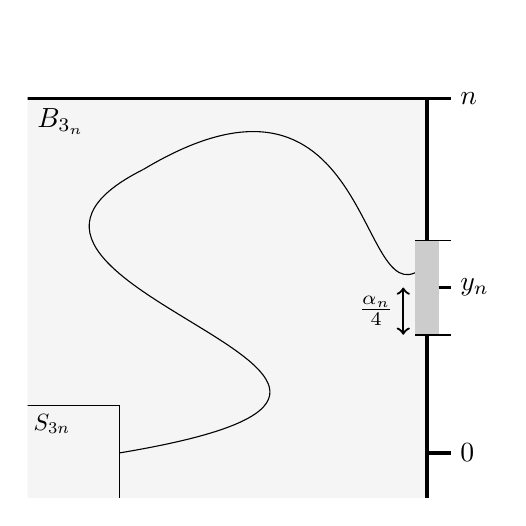
\begin{tikzpicture}[scale = 0.3]
				% Clip
				\clip 					(-1.9,-1.9)	rectangle	(18,18)	;
				% Fond
				\fill [color=gray!8]	(-15,-15)	rectangle	(15,15)	;	% B_n
				% Rectangles
				\draw 	[very thick]	(-15,-15)	rectangle 	(15,15) ;	%B_3n
				\draw 					(-2,-2) 	rectangle 	(2,2) 	;	%S_3n
				% Courbe de Bézier
				\draw (2, 0) 	.. controls (20, 3) and (-7, 7) 	.. (3, 12);
				\draw (3, 12) 	.. controls (13, 18) and (12, 5)	.. (15, 8);
				% Plage
				\fill [color=gray!40]	(14.5, 5) 	rectangle (15.5, 9);
				% Points
				\path [below right]	(-1.9, 15)	node				{$B_{3_n}$}	;
				\path [below right]	(-2, 2)		node	[scale=0.85]{$S_{3n}$}	;
				% Courbes de séparation
				\draw [very thick]	(15, 0)		-- (16, 0);
				\draw [very thick] 	(14, 15) 	-- (16, 15);
				\draw [thick]		(14.5, 5) 	-- (16, 5);
				\draw [thick]		(15.5, 7) 	-- (16, 7);
				\draw [right]		(14.5, 9) 	-- (16, 9);
				\draw [right]		(16, 0) 	node {$0$};
				\draw [right]		(16, 7)		node {$y_n$};
				\draw [right]		(16, 15) 	node {$n$};
				\draw[<->, thick]	(14, 5) 	-- (14, 7);
				\draw [left]		(14, 6)		node {$\frac{\alpha_n}{4}$};
			\end{tikzpicture}
		\end{center}
		\caption{Les événements~$\mathcal{E}_n(\alpha_n, n)$ et~$\mathcal{E}_n(y_n - \frac{\alpha_n}{4}, y_n + \frac{\alpha_n}{4})$}
		\label{fig:figuLemCollagesElem}
	\end{figure}

	Dans la preuve de ce lemme ainsi que dans la suite de l'article, on utilisera librement l'inégalité de Harris-FKG aussi bien sous sa forme classique que sous la forme suivante qui en est une conséquence immédiate. On en trouvera une preuve dans~\cite{Grimmett}. 
	\begin{lem}[square root trick]\label{lem:HarrisFKG}
		Soient~$A_1, A_2, \ldots, A_n$ des événements croissants ; alors
		\[
			\max_{1 \leq i \leq n} \Pp{A_i} \geq 1 - (1 - \Pp{A_1 \cup A_2 \cup \cdots \cup A_n})^{1/n}. 
		\]
	\end{lem}
	
	\begin{dem}[du lemme~\ref{lem:collagesElem}]
		En découpant le carré~$\partial B_n$ en ses~$8$ demi-côtés, on peut décomposer l'événement~$\relie[B_n]{S_n}{\partial B_n}$ en la réunion de~$8$ événements obtenus à partir de~$\mathcal{E}_n(0, n)$ en effectuant des rotations et des réflexions. L'invariance du modèle par lesdites réflexions et rotations permet d'affirmer que ces événements sont tous de même probabilité. On peut donc appliquer l'inégalité de Harris-FKG de la manière suivante
		\[
			\Pp{\mathcal{E}_n(0,n)} \geq 1 - \left(1 - \Pp{\relie[B_n]{S_n}{\partial B_n}} \right)^{1/8}.
		\]
		Ce qui donne,~$\Pp{\mathcal{E}_n(0, n)}$ tend vers 1 lorsque~$n$ tend vers l'infini. Sachant cela, on peut décomposer~$\mathcal{E}_n(0, n)$ en~$\mathcal{E}_n(0, \alpha) \cup \mathcal{E}_n(\alpha + 1, n)$. Il faut ensuite choisir pour chaque~$n$ un~$\alpha$ assez grand pour que la deuxième condition du lemme soit vérifiée mais suffisamment éloigné de~$n$ pour que la première condition reste vraie. En appliquant à nouveau Harris-FKG aux événements~$\mathcal{E}_n(0, 0)$ et~$\mathcal{E}_n(1, n)$, on obtient
		\[
			\max(\Pp{\mathcal{E}_n(0, 0)}, \Pp{\mathcal{E}_n(1, n)}) \xrightarrow[n \to \infty]{} 1.
		\]
		Or la probabilité de l'événement~$\mathcal{E}_n(0,0)$ est bornée uniformément par rapport à~$n$ par la constante~$1 - (1-p)^{3(k+1)}$ donc à partir d'un certain rang, la probabilité de~$\mathcal{E}_n(0,0)$ est inférieure à la probabilité de~$\mathcal{E}_n(1, n)$. On obtient de la même manière que la probabilité de~$\mathcal{E}_n(0, n-1)$ est inférieure à celle de~$\mathcal{E}_n(n, n)$ à partir d'un certain rang. Cela permet de poser
		\[
			\alpha_n = \max \{ \alpha \in \llbracket 0;n-1 \rrbracket, \Pp{\mathcal{E}_n(0, \alpha - 1)} < \Pp{\mathcal{E}_n(\alpha, n)} \}.
		\]
		Avec ce choix de~$\alpha_n$, et en appliquant l'inégalité de~Harris-FKG aux événements~$\mathcal{E}_n(0, \alpha_n)$ et~$\mathcal{E}_n(\alpha_n + 1, n)$ puis aux événements~$\mathcal{E}_n(0, \alpha_n - 1)$ et~$\mathcal{E}_n(\alpha_n, n)$, on peut minorer les probabilités des événements~$\mathcal{E}_n(0, \alpha_n)$ et~$\mathcal{E}_n(\alpha_n, n)$ par~$1 - \sqrt{1  - \Pp{\mathcal{E}_n(0, n)}}$ ; ce qui donne leur convergence vers~$1$. 

		On cherche maintenant à trouver~$y_n$, pour cela on effectue d'abord la décomposition~$\mathcal{E}_n(0, \alpha_n) = \mathcal{E}_n(0, \alpha_n/2) \cup \mathcal{E}_n(\alpha_n/2, \alpha_n)$. Et il suffit alors de choisir~$y_n$ égal à $\alpha_n/4$ ou~$3\alpha_n/4$ de sorte à maximiser la probabilité de~$\mathcal{E}_n(y_n - \alpha_n/4, y_n + \alpha_n/4)$. Par une dernière application de l'inégalité de Harris-FKG, on obtient enfin à partir d'un certain rang que
		\[
			\Pp{\mathcal{E}_n\left(y_n - \frac{\alpha_n}{4}, y_n + \frac{\alpha_n}{4}\right)}
					\geq 1 - \sqrt{1 - \Pp{\mathcal{E}_n(0, \alpha_n)}}.
		\]
		Ce qui permet de conclure que ces choix de~$y_n$ et~$\alpha_n$ conviennent.
	\end{dem}
	Pour la suite, on pose~$\suite{\alpha}$ et~$\suite{y}$ des suites vérifiant les hypothèses du lemme~\ref{lem:collagesElem}. On définit maintenant quelques ensembles utiles, qui seront illustrés dans la figure~\ref{fig:illuEvent}.
	\begin{align*}
		&B_n' = (2n, y_{3n}) + B_n \marginnote{$B_n'$} \\
		&S_n' = (2n, y_{3n}) + S_n \marginnote{$S_n'$} \\
		&Y_n^+ = {3n} \times [y_{3n} + \alpha_n; y_{3n} + n] \marginnote{$Y_n^+$} \\
		&Y_n^- = {3n} \times [y_{3n} - n; y_{3n} - \alpha_n] \marginnote{$Y_n^-$} \\
		&Z_n = {3n} \times [y_{3n} - \alpha_n; y_{3n} + \alpha_n] \marginnote{$Z_n$}
	\end{align*}
	\vfill{}
	\begin{figure}[h]
		\begin{center}
		\begin{quartCarre}
			%Courbes de Bézier 1
			%\draw 	[thick]	(0,2) 	.. controls (0,6) 		and (-3,10) .. (3,10);
			%\draw 	[thick]	(3,10)	.. controls (6,10) 		and (5,7) 	.. (7,5);
			%\draw	[thick]	(7,5)		.. controls (9,3)		and (13,6) 	.. (15,7.5);
			%Courbe de Bézier 2	
			%\draw	[thick, color=gray!85]	(9,8)		.. controls (8,8)		and (8,8) 	.. (7,5);
			%\draw	[thick, color=gray!85]	(7,5)		.. controls (6,2)		and (13,5)	.. (15, 5);
			%Courbe de Bézier 3
			%\draw 	[thick, color=gray!85]	(10.5,9)	.. controls (9.5,12)	and (12,14)	.. (15,11);
			%Plages
			\fill [color=gray!40]	(14.5,3)	rectangle (15.5,6);
			\fill [color=gray!40]	(14.5,10)	rectangle (15.5,13);
			\fill [color=gray!8]	(14.5,6)	rectangle (15.5,10);
			\fill [pattern=north east lines]	(14.5,6)	rectangle (15.5,10);
			%Text + barres de séparation
			\draw [thick]	(5,3) 		-- (16,3);
			\draw [thick]	(5,13)		-- (16,13);
			\draw 			(14.5, 6)	-- (16,6);
			\draw 			(14.5, 6)	-- (16,6);
			\draw 			(14.5, 10)	-- (16,10);
			\path	[right]	(15.5, 8)		node	{$Z_n$}	;
			\path	[right]	(15.5, 4.5)		node	{$Y_n^+$}	;
			\path	[right]	(15.5, 11.5)	node	{$Y_n^-$}	;
		\end{quartCarre}
		\end{center}
		\caption{Illustration des ensembles~$B_n', S_n',Y_n^+,Y_n^-$ et~$Z_n$.}
		\label{fig:illuEvent}
	\end{figure}
	On souhaite d'abord relier~$S_{3n}$ à~$Z_n$ ainsi que $S_n'$ à~$Y_n^+$ et~$Y_n^-$. Le lemme gluant (lemme~\ref{lem:gluant}) permettra ensuite de lier~$S_{3n}$ à~$S_n'$. On a pour tout~$n$, $\alpha_n \leq n$ donc il existe une infinité de~$n$ tels que~$\alpha_{3n} \leq 4\alpha_n$ car sinon, à partir d'un certain rang, la suite aurait une croissance sur-linéaire, ce qui est impossible. Quand~$\alpha_{3n} \leq 4\alpha_n$, on a
	\[
		\Pp{\relie[B_{3n}]{S_{3n}}{Z_n}} \geq \Pp{\mathcal{E}_{3n}\left(y_{3n} - \frac{\alpha_{3n}}{4}, y_{3n} + \frac{\alpha_{3n}}{4}\right)}.
	\]

	Ainsi par la remarque précédente et le lemme~\ref{lem:collagesElem}, la limite supérieure de la suite de probabilités~$\Pp{\relie[B_{3n}]{S_{3n}}{Z_n}}$ tend vers~$1$ quand~$n$ tend vers l'infini. Maintenant que nous avons relié~$S_{3n}$ à~$Z_n$, ajoutons y~$Y_n^+$ et~$Y_n^-$. On obtient à l'aide de Harris-FKG
	\[
		\Pp{\relie[B_{3n}]{S_{3n}}{Z_n}, \relie[B_n']{S_n'}{Y_n^+}, \relie[B_n']{S_n'}{Y_n^-}} \geq \Pp{\relie[B_{3n}]{S_{3n}}{Z_n} }\Pp{\mathcal{E}_n(0, \alpha_n)}^2.
	\]
	On a donc enfin
	\[ 
		\limsup_{n \to \infty} \Pp{\relie[B_{3n}]{S_{3n}}{Z_n}, \relie[B_n']{S_n'}{Y_n^+}, \relie[B_n']{S_n'}{Y_n^-}} = 1.
	\]


